\documentclass{article}

\textwidth=6.5in
\textheight=8.5in
\voffset=-54pt
\oddsidemargin=0in
\evensidemargin=0in
\setlength{\parskip}{8pt}
\setlength{\parindent}{0pt}

\usepackage{amsmath, amssymb}
\usepackage{ifthen}

\usepackage[inline]{enumitem}
\setlist{topsep=0pt, parsep=8pt}

\usepackage[rgb,table]{xcolor}\convertcolorsUfalse
\usepackage{graphicx}

% change hyperref options
\PassOptionsToPackage{hyphens}{url}
\usepackage[bookmarks,colorlinks,linkcolor=black,citecolor=blue,pdfstartview=FitH,urlcolor=blue]{hyperref}
\hypersetup{pdfpagemode=UseNone}
\usepackage{bookmark}

\usepackage{graphicx}
\usepackage{multicol}
\usepackage{framed}
\usepackage{array}

\usepackage{icomma}

%
\providecommand{\topic}{}
\renewcommand{\topic}[1]{}

\usepackage{pifont}

\newlist{altenumerate}{enumerate}{3}

\usepackage{soul}

\usepackage{pgfplots}
\pgfplotsset{compat=1.18}  
\pgfplotscreateplotcyclelist{mycolor}{black, blue, red, green!70!black, magenta, purple, cyan, orange }  
\pgfplotsset{
  disabledatascaling,
  cycle list=tikzcolor, 
  axis lines=middle,
  every axis plot/.style={no marks, thick},
  every axis/.style={
    enlarge x limits=false,
    enlarge y limits=auto,
    xlabel style={at={(current axis.right of origin)},anchor=west},
    ylabel style={at={(current axis.above origin)},anchor=south},
    % extra x and y ticks for asymptotes
    extra x tick style={grid=major, grid style={dashed,black}},
    extra y tick style={grid=major, grid style={dashed,black}},
    /pgf/number format/1000 sep={},
  },    
  tick label style = {font=\footnotesize, fill=\currentbgcolor, inner sep=0pt},    
  xticklabel shift=1pt,    
  scaled ticks=false,
  scaled y ticks=false,
  unbounded coords=jump,
  samples=101,
  minor tick length=0,
  scatter/classes={
    open={mark=*,draw=black,fill=white, mark size=2, thin},
    closed={mark=*,draw=black,fill=black, mark size=2, thin}
  },
  width=3in,
}
\pgfplotsset{open/.style={only marks, mark=*, fill=white, thin, mark size=2}}
\pgfplotsset{closed/.style={only marks, mark=*, draw=black, fill=black,
    thin, mark size=2}}
\pgfplotsset{labeled/.style={nodes near coords, only marks, mark=*, draw=black, fill=black, thin, mark size=2, point meta=explicit symbolic}}

\pgfplotsset{gridgraph/.style={clip=false, axis line style={shorten
      >=-8pt}, xlabel style={xshift=8pt}, ylabel style={yshift=8pt},
    enlargelimits=false, grid=major, tick style={black}}} 

\newcommand{\axes}[1][]{
  \begin{tikzpicture}
    \begin{axis}[xtick=\empty, ytick=\empty, ymin=-2, ymax=2,
      xmin=-4.25, xmax=4.25, #1]
    \end{axis}
  \end{tikzpicture}
}
\usepackage{tikz}
\usetikzlibrary{
  matrix,%
  % enables the snake paths
  decorations.pathmorphing,%
  % enables bigger arrows
  decorations.markings,%
  decorations.pathreplacing,%
  decorations.text,%
  calc,%
  patterns,%
  shapes.geometric,%
  arrows,
  decorations.shapes,
  positioning,
  plotmarks,
  intersections
}
\tikzset{>=latex} % sets default arrow type in tikz
\tikzset{font=\normalsize}
\tikzset{mark size=1.5pt, mark options=thin}
\tikzset{pin distance=4pt,
  every pin edge/.style={<-, thin, shorten <= -2pt}}

\interfootnotelinepenalty=10000
\renewcommand{\thefootnote}{(\arabic{footnote})}

\usepackage{multirow, bigdelim}

% change to \usepackage[sols]{handout} to see solutions
\usepackage{handout}

\newcommand\iscurrentenumi[1]{%
  \ifthenelse{\equal{#1}{\theenumi}}{}{#1}}
\setenumerate[1]{ref=\#\arabic*}
\setenumerate[2]{ref=\protect\iscurrentenumi{\theenumi}(\alph*)}
\newcommand\enumiiprefix[2]{%
  \ifthenelse{{\equal{#1}{\theenumi}}\AND{\equal{#2}{(\alph{enumii})}}}{}{}%
  \ifthenelse{{\equal{#1}{\theenumi}}\AND{\NOT{\equal{#2}{(\alph{enumii})}}}}{#2}{}%
  \ifthenelse{\equal{#1}{\theenumi}}{}{#1#2}%
}
\setenumerate[3]{ref=\protect\enumiiprefix{\theenumi}{(\alph{enumii})}\roman*}

\makeatletter

% underline links               
\let\@href=\href
\renewcommand{\href}[2]{\@href{#1}{\ul{#2}}}

\newdimen\SOUL@dimen %new
\def\SOUL@ulunderline#1{{%
    \setbox\z@\hbox{#1}%
    % \dimen@=\wd\z@
    \SOUL@dimen=\wd\z@ %new
    \dimen@i=\SOUL@uloverlap
    \advance\SOUL@dimen2\dimen@i %\dimen@ exchanged too
    \rlap{%
      \null
      \kern-\dimen@i
      % \SOUL@ulcolor{\SOUL@ulleaders\hskip\dimen@}%
      \SOUL@ulcolor{\SOUL@ulleaders\hskip\SOUL@dimen}% new
    }%
    \unhcopy\z@
  }}

\makeatother

\newcommand{\related}[1]{%
\fcolorbox{black}{yellow}{%
  %\parbox[t]{12pt}{$\clubsuit$}%
  \parbox[t]{\linewidth-8pt}{\emph{Related problems:} #1}}}

\renewcommand{\answer}[1]{#1}

\definecolor{purple}{rgb}{0.5,0,1.0}
\definecolor{hotpink}{rgb}{1, 0, 0.5}

\definecolor{skyblue}{rgb}{0, 0.5, 1}

\newcommand{\highlight}[1]{\boldmath\hl{\textbf{#1}}\unboldmath}

\newcommand{\goal}[1]{\textbf{\textcolor{skyblue}{#1}}}

\usepackage{amsthm}

% make URLs print in the same font
\usepackage{url}
\urlstyle{same}

\usepackage{pifont}
\def\exend{\hfill\ding{118}}

%\makeatletter\@addtoreset{equation}{section}\makeatother
%\renewcommand{\theequation}{\arabic{section}.\arabic{equation}}

\newtheoremstyle{theorem}% name
{8pt}%      Space above
{0pt}%      Space below
{\itshape}%         Body font
{}%         Indent amount (empty = no indent, \parindent = para indent)
{\bfseries}% Thm head font
{.}%        Punctuation after thm head
{.5em}%     Space after thm head: " " = normal interword space;
                                %       \newline = linebreak
{}%         Thm head spec (can be left empty, meaning `normal')

\theoremstyle{theorem}

\let\Theorem\undefined
\newtheorem{Theorem}[equation]{Theorem}
\let\Definition\undefined
\newtheorem{Definition}[equation]{Definition}
\let\Summary\undefined
\newtheorem{Summary}[equation]{Summary}
\let\Conjecture\undefined
\newtheorem{Conjecture}[equation]{Conjecture}
\let\Fact\undefined
\newtheorem{Fact}[equation]{Fact}

\renewcommand{\thesubsection}{\arabic{subsection}}
\makeatletter
\def\@seccntformat#1{\@ifundefined{#1@cntformat}%
   {\csname the#1\endcsname\quad}%       default
   {\csname #1@cntformat\endcsname}}%    enable individual control
\newcommand\section@cntformat{}
\makeatother

  \usepackage{exam}

\usepackage{fancyhdr}
\lhead{\textcolor{white}{This content is protected and may not be shared, uploaded, or distributed.}}
\rhead{}
\rfoot{\vspace*{\fill}\footnotesize\textcopyright{} \emph{Harvard Math Ma}}
\renewcommand{\headrulewidth}{0pt}
\pagestyle{fancy}
\begin{document}

  \title{Final Exam Practice 1}

\instructions{instructions.tex}{}

\listofproblems

\begin{enumerate}
\item \points{15} \label{fall2014-m2practice-exp-graphing} 

  \topic{graphing, exponentials}

  Let $f(x) = e^x (3 - e^{2x})$.  

  \begin{enumerate}
  \item
    \begin{problem}[1in]
      What are the discontinuities of $f(x)$? Classify each as a removable discontinuity, jump discontinuity, or vertical asymptote.
    \end{problem}

    \begin{solution}
      $f$ is made up of familiar functions, so it's discontinuous where it's undefined. But $f$ is never undefined, so it has \fbox{no discontinuities}.
    \end{solution}

  \item
    \begin{problem}[\vfill]
      Does $f$ have any horizontal asymptotes?  If so, what are they? Justify your answer completely. 
    \end{problem}

    \begin{solution}
      We answer this by calculating $\displaystyle \lim_{x \to \infty} f(x)$ and $\displaystyle \lim_{x \to -\infty} f(x)$. As $x \to \infty$, $e^x \to \infty$ and $3 - e^{2x} \to -\infty$, so $\boxed{ \lim_{x \to \infty} f(x) = - \infty}$. As $x \to -\infty$, $e^x \to 0$ and $3 - e^{2x} \to 3$, so $\boxed{ \lim_{x \to -\infty} f(x) = 0}$. So, \fbox{there is only horizontal asymptote, $y = 0$}.
    \end{solution}

  \item
    \begin{problem}[\vfill\newpage]
      Find all $x$- and $y$-intercepts of $f$. 
    \end{problem}

    \begin{solution}
      The \fbox{$y$-intercept is at $f(0) = 2$}.

      To find the $x$-intercepts, we solve $e^x (3 - e^{2x}) = 0$. This happens when $e^x = 0$ (never) or when $e^{2x} = 3$.
      \begin{align*}
        e^{2x} &= 3 \\
        \intertext{Taking the natural log of both sides,}
        2x &= \ln 3 \\
        x &= \frac{\ln 3}{2}
      \end{align*}
      So, $f$ has an \fbox{$x$-intercept at $\frac{\ln 3}{2}$}.
    \end{solution}

  \item 
    \begin{problem}[\stretch{3}]
      On what intervals is $f$ increasing?  
    \end{problem}

    \begin{solution}
      We can figure this out by making a sign chart for $f'$. First, we can rewrite $f(x) = 3 e^x - e^{3x}$, so $f'(x) = 3 e^x - 3 e^{3x}$. This is always defined, and it is 0 when
      \begin{align*}
        3 e^x &= 3 e^{3x} \\
        e^x &= e^{3x} \\
        1 &= \frac{e^{3x}}{e^x} = e^{2x} \\
        \intertext{Taking the natural log of both sides,}
        \ln 1 &= 2x \\
        0 &= 2x \\
        0 &= x
      \end{align*}
      So, the only critical number is $x = 0$. Now, we test points; for example,
      \begin{align*}
        f'(-1) &= 3 e^{-1} - 3 e^{-3} > 0 \\
        f'(1) &= 3 e - 3e^3 < 0 
      \end{align*}
      So, here's a sign chart for $f'$:
      \begin{center}
        \begin{tikzpicture}
          \begin{axis}[axis y line=none, x axis line style={-}, xtick={0}, ymin=-2, height=1in, width=3in, clip=false]
            \addplot+[domain=-0.2:0.1, very thin]{0};
            \draw (axis cs: -0.2, -1.5) node[right] {sign of $f'$};
            \draw (axis cs: -0.05, -1.5) node{$+$};
            \draw (axis cs: 0.05, -1.5) node{$-$};
          \end{axis}
        \end{tikzpicture}
      \end{center}
      So, $f$ is increasing on $\boxed{(-\infty, 0)}$. 
    \end{solution}

  \item 
    \begin{problem}[\vfill\newpage]
      Your friend has correctly found that $f$ has exactly one inflection point at $x = \dfrac{1}{2} \ln \left( \dfrac{1}{3} \right)$. Use this, together with what you found in (a) - (d), to sketch the graph of $f$. Please label the $x$-values of any turning points, inflection points, or $x$-intercepts. 
    \end{problem}

    \begin{solution}
      Remember that an inflection point is a point where $f$ changes concavity. We're told there's only one such point. Since $\displaystyle \lim_{x \to -\infty} f(x) = 0$, the graph of $f$ must be concave up when $x$ is very negative. So, it must be the case that $f$ is concave up on $\left( 0, \dfrac{1}{2} \ln \left( \dfrac{1}{3} \right) \right) $ and concave down on $\left( \dfrac{1}{2} \ln \left( \dfrac{1}{3} \right), \infty \right)$.

      Notice that $\ln \left( \frac{1}{3} \right)$ is negative.\footnote{You can figure this out by thinking about the graph of $\ln x$ or by thinking about $\ln \left( \frac{1}{3} \right)$ as the power we must raise $e$ to in order to get $\frac{1}{3}$.} So, here's a sketch of $f$:
      \begin{center}
        \answer{
          \begin{tikzpicture}
            \begin{axis}[ymin=-10, xtick={-0.5493, 0.5493},
              xticklabels={$\frac{1}{2} \ln \left( \frac{1}{3} \right)$,
                $\frac{\ln 3}{2}$}, ytick={2}] 
              \addplot+[domain=-2:2] {e^x*(3-e^(2*x))};
            \end{axis}
          \end{tikzpicture}
        }
      \end{center}
    \end{solution}

    \begin{grading}
      The main thing we're looking for in your graph is consistency with the previous parts and the given information. So, the key features are:
      \begin{itemize}
      \item The graph is increasing on $(-\infty, 0)$ and decreasing on $(0, \infty)$.
      \item The graph has a $y$-intercept at $(0, 2)$ and an $x$-intercept at $\left( \frac{\ln 3}{2}, 0 \right)$. (It has no other $x$-intercepts.)
      \item $\displaystyle \lim_{x \to -\infty} f(x) = 0$ and $\displaystyle \lim_{x \to \infty} f(x) = -\infty$.
      \item The graph is concave up on $\left( - \infty, \frac{1}{2} \ln \left( \frac{1}{3} \right) \right)$ and concave down on $\left( \frac{1}{2} \ln \left( \frac{1}{3} \right), \infty \right)$, so there is an inflection point at $x = \frac{1}{2} \ln \left( \frac{1}{3} \right)$.
      \end{itemize}
    \end{grading}

  \end{enumerate}

\item \label{fall20112-prefinal-practice3-6-modified} \points{15}  

  A zookeeper is tracking the weight of a tiger cub. One week after the cub is born, it weighs 3 kg. Three weeks after it's born, it weighs 12 kg. 

  \begin{enumerate}
  \item
    \begin{problem}[\stretch{0.75}]
      Write a function $C(t)$ that gives the tiger's weight $t$ weeks after birth if its weight is increasing at a \emph{constant} rate.
    \end{problem}

    \begin{solution}
      The graph of $C(t)$ is the line through the points $(1, 3)$ and $(3, 12)$. That line has slope $\dfrac{12-3}{3-1}=\dfrac{9}{2}$. Since it goes through the point $(1, 3)$, we can write its equation in point-slope form as $C - 3 = \dfrac{9}{2}(t - 1)$. So, $C(t) = \boxed{3 + \frac{9}{2}(t - 1)} = \dfrac{9}{2} t - \dfrac{3}{2}$.
    \end{solution}

  \item
    \begin{problem}[\vfill]
      Suppose instead that the tiger's weight is an exponential function of time. Write a function $E(t)$ that gives the tiger's weight $t$ weeks after birth in this scenario. 
    \end{problem}

    \begin{solution}
      Now, we want an exponential function through the points $(1, 3)$ and $(3, 12)$. We know every exponential function can be expressed as $E(t) = C \cdot b^t$ for some $C, b$ or as $E(t) = C e^{kt}$ for some $C, k$. You can use either form to solve the problem; here, we'll use the first.

      We have
      \begin{alignat*}{3}
        E(1) &= 3 & \implies & C \cdot b^1 &= 3 \\
        E(3) &= 12 & \implies & C \cdot b^3 &= 12 
      \end{alignat*}
      Dividing the second equation by the first, $\dfrac{12}{3} = \dfrac{C \cdot b^3}{C \cdot b^1} = b^2$, so $b = 2$.

      Plugging $b = 2$ into the first equation gives $C \cdot 2 = 3$, so $C = \dfrac{3}{2}$.

      Therefore, $E(t) = \boxed{\frac{3}{2} \cdot 2^t}$. 
    \end{solution}

  \item
    \begin{problem}[\nstretch{1.5}]
      On a single set of axes, sketch a large graph of $C(t)$ and $E(t)$, making sure to reflect the information given in the problem. Please indicate the units of each axis. 
    \end{problem}

    \begin{solution}
      Both graphs should pass through $(1, 3)$ and $(3, 12)$. The graph of $C$ is linear, while the graph of $E$ is an exponential growth function.
      \begin{center} 
        \answer{
          \begin{tikzpicture}
            \begin{axis}[ymin=0, ytick={3, 12}, xtick={1, 3}, clip=false, xlabel={$t$ (weeks)}, ylabel={weight (kg)}]
              \addplot[closed] coordinates{(1, 3)}; %
              \addplot[closed] coordinates{(3, 12)}; %
              \addplot+[domain=0:3.5] [skyblue]{9/2*x-3/2} node[right]{$y = C(t)$}; %
              \addplot+[domain=0:3.5] [hotpink]{3/2*2^x} node[anchor=south west]{$y = E(t)$}; %
            \end{axis}
          \end{tikzpicture}
        }
      \end{center}
    \end{solution}

  \item
    \begin{problem}[\vfill]
      Which is larger, $C(2)$ or $E(2)$? Explain briefly. 
    \end{problem}

    \begin{solution}
      From the graph, we see that \fbox{$C(2)$} is larger. 
    \end{solution}

  \item
    \begin{problem}[\vfill]
      Which is larger, $C(7)$ or $E(7)$? Explain briefly. 
    \end{problem}

    \begin{solution}
      From the graph, we see that, when $t > 3$, $E(t) > C(t)$. So, \fbox{$E(7)$} is larger.
    \end{solution}

  \item
    \begin{problem}[\vfill]
      Which is larger, $C'(1)$ or $E'(1)$? Explain.
    \end{problem}

    \begin{solution}
      From the graph, we can see that the slope of the tangent line to $y = C(t)$ at $t = 1$ is greater than the slope of the tangent line to $y = E(t)$ at $t = 1$, so \fbox{$C'(1)$} is larger. 
    \end{solution}

  \item

    \begin{problem}[\nstretch{2}]
      Is there a time when $E'(t)=C'(t)$? If so, find this time, and sketch what it means to have $E'(t) = C'(t)$ on the graph you sketched above. If not, explain why not. 
    \end{problem}

    \begin{solution}
      At a point somewhere between $t=1$ and $t=3$, the tangent line to $E(t)$ becomes parallel to the line $C(t)$, and at this point $E'(t)=C'(t)$:
      \begin{center} 
        \begin{tikzpicture}
          \begin{axis}[ymin=0, ytick={3, 12}, xtick={1, 2.11, 3}, xticklabels={1, ?, 3}, clip=false, xlabel={$t$ (weeks)}, ylabel={weight (kg)}]
            \addplot[closed] coordinates{(1, 3)}; %
            \addplot[closed] coordinates{(3, 12)}; %
            \addplot+[domain=0:3.5] [skyblue]{9/2*x-3/2} node[right]{$y = C(t)$}; %
            \addplot+[domain=0:3.5] [hotpink]{3/2*2^x} node[anchor=south west]{$y = E(t)$}; %
            \addplot+[closed] coordinates { ({ln(3/ln(2))/ln(2)}, {9/(2*ln(2))}) };
            \addplot+[domain=1.11:3.11, green!90!black] {9/2*(x-2.11)+9/(2*ln(2))}; 
          \end{axis}
        \end{tikzpicture}
      \end{center}
      Let's find this time. Differentiating our formulas for $C(t)$ and $E(t)$, we have $C'(t) = \dfrac{9}{2}$ and $E'(t) = \dfrac{3}{2} \cdot 2^t \ln 2$. We set these equal to each other:
      \begin{align*}
        \frac{3}{2} \cdot 2^t \ln 2 &= \frac{9}{2} \\
        2^t &= \frac{3}{\ln 2} \\
        t &= \boxed{\log_2 \left( \frac{3}{\ln 2} \right)}
      \end{align*}
      (This value is approximately $2.11$.)
    \end{solution}

  \end{enumerate}

\item \points{7} 

  In each part, you're given a scenario. Decide which type of function we've learned about (linear, quadratic, exponential, logarithmic, etc.) is most appropriate for modeling the scenario. No explanation is necessary. 

  \begin{enumerate}
  \item
    \begin{problem}[\vfill]
      A recent study of microplastic pollution found that \href{https://www.wired.com/story/the-microplastic-crisis-is-getting-exponentially-worse/}{``microplastic levels have been doubling in Arctic Ocean sediments every 23 years''}. What kind of function expresses microplastic levels as a function of time? 
    \end{problem}

    \begin{solution}
      Since the microplastic level gets multiplied by the same factor (2) every 23 years, this is modeled by an \answer{exponential} function.
    \end{solution}

  \item
    In the science fiction novel \emph{Project Hail Mary} by Andy Weir, the protagonist's spaceship travels at a constant acceleration.

    \solonly{\related{{{\#1}} on \href{https://people.math.harvard.edu/~jjchen/mathma/docs/worksheets/worksheet34-sols.html}{the worksheet ``Quadratics''}; \href{https://people.math.harvard.edu/~jjchen/mathma/docs/homework/PS34.html}{Problem Set 34}, {{\#2}}}}

    \begin{enumerate}
    \item
      \begin{problem}[\vfill]
        What kind of function best expresses the spaceship's velocity as a function of time? 
      \end{problem}

      \begin{solution}
        Let's write $v(t)$ for the velocity at time $t$. Acceleration is the derivative of velocity, so $v'(t)$ is constant. This means the graph of $v(t)$ has constant slope, so $v(t)$ must be \fbox{linear}. 
      \end{solution}

    \item
      \begin{problem}[\vfill]
        What kind of function best expresses the spaceship's position as a function of time? 
      \end{problem}

      \begin{solution}
        If we write $f(t)$ for the spaceship's position at time $t$, then $f'(t)$ is the velocity at time $t$. So, $f'(t)$ is a linear function, say $f'(t) = mt + b$. Working backwards, we see that $f(t)$ must be a \fbox{quadratic} function. 
      \end{solution}

    \end{enumerate}

  \item
    \begin{problem}[\vfill]
      Sound levels are measured in decibels. For example, the noise level in a typical office is around 70 decibels, while the noise level at a typical rock concert is around 110 - 120 decibels. An increase of 1 decibel corresponds to the noise being 1.26 times as loud. What kind of function best expresses decibels as a function of loudness?
    \end{problem}

    \begin{solution}
      Since each increase by 1 decibel multiplies the loudness by the same factor, loudness is an exponential function of decibels. But we want decibels as a function of loudness. That's the inverse function of the exponential function we just described, and the inverse of an exponential function is \fbox{logarithmic}. 
    \end{solution}    

  \item
    \begin{problem}[\vfill\newpage]
      After a drug is administered to a patient via an IV, the patient starts metabolizing the drug. This causes the concentration of drug in their bloodstream to decrease at a rate proportional to the amount of drug in their bloodstream. What kind of function best expresses the drug concentration as a function of time? 
    \end{problem}

    \begin{solution}
      As we saw in \href{https://people.math.harvard.edu/~jjchen/mathma/docs/worksheets/worksheet24-sols.html}{the worksheet ``Derivatives of Exponential Functions''}, only \fbox{exponential} functions have the property that the derivative of the function is proportional to the function itself.
    \end{solution}

  \end{enumerate}

\item \points{8} 

  In each part, decide whether there is a polynomial with the specified properties. If so, give the equation of an example and explain briefly how you know it has the specified properties. If there is no such polynomial, explain why.

  \begin{enumerate}

  \item
    \begin{problem}[\vfill]
      A polynomial with 6 roots and 4 turning points. 
    \end{problem}

    \begin{solution}
      Between any two consecutive roots, the polynomial must switch from increasing to decreasing or vice versa (for example, if the polynomial is decreasing when it goes through one root, it needs to ``turn around'' to reach the next root). Therefore, a polynomial with 6 roots must have at least 5 turning points, so this is \fbox{impossible}. 
    \end{solution}

  \item
    \begin{problem}[\vfill\newpage]
      A degree 5 polynomial with no $x$-intercepts.
    \end{problem}

    \begin{solution}
      If $p(x)$ is a degree 5 polynomial, then either $\displaystyle\lim_{x \to \infty} p(x)=\infty$ and $\displaystyle\lim_{x \to -\infty} p(x) = -\infty$, or $\displaystyle\lim_{x \to \infty} p(x)=-\infty$ and $\displaystyle\lim_{x \to -\infty} p(x)=\infty$. In either case, there are some values of $x$ where $p(x)$ is positive and some values of $x$ where $p(x)$ is negative. Since a polynomial is continuous everywhere, the graph of $p(x)$ must be 0 somewhere between when it's positive and when it's negative. So, this is \fbox{impossible}.
    \end{solution}

  \item
    \begin{problem}[\nstretch{1.25}]
      A cubic with turning points at $x=1$ and $x=3$.
    \end{problem}

    \begin{solution}
      Graphically, we can see that this should be possible:
      \begin{center}
        \begin{tikzpicture}
          \begin{axis}[xtick={1, 3}, ytick=\empty, width=2.25in]
            \addplot+[domain=-0.3:4.3] {x^3/3-2*x^2+3*x+1}; 
          \end{axis}
        \end{tikzpicture}
      \end{center}
      Let's come up with an example $f(x)$. Since $f$ has turning points at $x=1$ and $x=3$, we need $f'(x)$ to change sign at $x = 1, 3$. Since $f(x)$ is a cubic, $f'(x)$ must be a quadratic. So, let's start by making up a possible $f'(x)$; we want a quadratic that's 0 when $x = 1, 3$. One example is $f'(x) = (x - 1)(x - 3) = x^2 - 4x + 3$, and this really does change sign at $x = 1, 3$:
      \begin{center}
        \begin{tikzpicture}
          \begin{axis}[xtick={1, 3}, ytick=\empty, width=1.75in]
            \addplot+[domain=-0.3:4.3] {x^2-4*x+3}; % 
          \end{axis}
        \end{tikzpicture}
      \end{center}
      So, we now just want to think of a function $f(x)$ whose derivative is $x^2 - 4x + 3$. Working backwards, \fbox{one example is $f(x) = \dfrac{x^3}{3} - 2x^2 + 3x$}.
    \end{solution}

  \end{enumerate}

\item \label{optimization-painted-vase} \points{13} 

  \begin{problem}
    Rosalyn plans to buy a cylindrical vase (shaped like a can with no top) whose volume is $160 \pi$ cm$^3$. She will paint the outside of the vase blue (just the sides, not the bottom), and then she'll paint the rim (the heavy dark line in the picture) gold. She determines that the blue paint will cost 2 cents per cm$^2$, and the gold paint will cost 20 cents per cm. If Rosalyn wants to minimize the cost of the paint, what dimensions should the vase be?

    Please communicate your reasoning clearly, and organize your work so the reader can follow it easily.
  \end{problem}

  \begin{problemonly}
    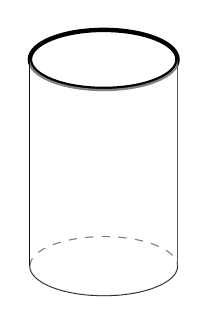
\begin{tikzpicture}[x=0.75cm, y=0.75cm]
      \draw[ultra thick] (0,0) ellipse (1.25 and 0.5);%
      \draw (-1.25,0) -- (-1.25,-3.5);%
      \draw (-1.25,-3.5) arc (180:360:1.25 and 0.5);%
      \draw [dashed] (-1.25,-3.5) arc (180:360:1.25 and -0.5);%
      \draw (1.25,-3.5) -- (1.25,0);%
      \fill [white,opacity=0.5] (-1.25,0) -- (-1.25,-3.5) arc (180:360:1.25 and 0.5) -- (1.25,0) arc (0:180:1.25 and -0.5);%
    \end{tikzpicture}
  \end{problemonly}

  \pspace{\newpage}

  \begin{solution}
    \highlight{Goal:} Minimize \goal{cost of paint}

    \highlight{Define variables:}
    \begin{itemize}[nosep]
    \item \goal{$C$ = cost of paint}
    \item $r$ = radius, $h$ = height
    \end{itemize}

    \begin{center}
      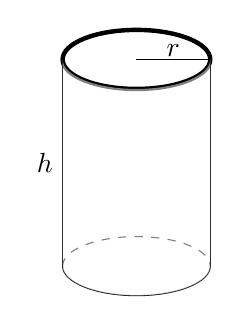
\begin{tikzpicture}[x=0.75cm, y=0.75cm]
        \draw[ultra thick] (0,0) ellipse (1.25 and 0.5);
        \draw (0, 0) -- node[above, inner sep=1pt]{$r$} (1.25, 0);
        \draw (-1.25,0) -- node[left]{$h$} (-1.25,-3.5);
        \draw (-1.25,-3.5) arc (180:360:1.25 and 0.5);
        \draw [dashed] (-1.25,-3.5) arc (180:360:1.25 and -0.5);
        \draw (1.25,-3.5) -- (1.25,0);  
        \fill [white,opacity=0.5] (-1.25,0) -- (-1.25,-3.5) arc (180:360:1.25 and 0.5) -- (1.25,0) arc (0:180:1.25 and -0.5);
      \end{tikzpicture}
    \end{center}

    \highlight{Formula for goal:}
    \begin{align*}
      \goal{$C$} &= \text{cost of blue paint} + \text{cost of gold paint} \\
      &= (2 \text{ cents/cm$^2$})(\text{surface area of blue paint}) + (20 \text{ cents/cm})(\text{length of gold paint}) \\
      &= 2 (2 \pi r h) + 20 (2 \pi r) \\
      &= 4 \pi r h + 40 \pi r
    \end{align*}
    This formula involves both $r$ and $h$, so we need to \highlight{relate $r$ and $h$ using something else we're told in the problem.}
    \begin{align}
      \text{volume of vase} &= 160 \pi \nonumber \\
      \pi r^2 h &= 160 \pi \nonumber \\
      r^2 h &= 160 \nonumber \\
      h &= \frac{160}{r^2} \label{eq:optimization-painted-vase}
    \end{align}
    Plugging this into our formula for $C$ gives $C$ as a function of just
    $r$,
    \[ \goal{$C(r)$} = 4 \pi r \cdot \frac{160}{r^2} + 40 \pi r = 40 \pi ( 16 r^{-1} + r).\]%
    \highlight{Critical points:} $\displaystyle C'(r) = 40 \pi (- 16r^{-2} + 1) = 40 \pi \left( 1 - \dfrac{16}{r^2} \right)$. This is undefined when $r = 0$, and it's 0 when 
    \begin{align*}
      1 &= \frac{16}{r^2} \\
      r^2 &= 16 \\
      r &= \pm 4
    \end{align*}
    But the only sensible values of $r$ are $r > 0$, so the only critical point in the domain is $r = 4$.

    \highlight{Global minimum:} Since there's only one critical point in the domain, we can try the First or Second Derivative Test. Let's try the Second Derivative Test, since it's easy to calculate that $C''(r) = 40 \pi (32 r^{-3}) = 40 \pi \cdot \dfrac{32}{r^3}$. Then, $C''(4) = 40 \pi \cdot \dfrac{32}{4^3} > 0$, so $C(r)$ has a local minimum at $r = 4$. Since this was the only critical point in the domain, this must be the global minimum.

    \highlight{Answer the question:} We can plug $r = 4$ into (\ref{eq:optimization-painted-vase}) to find that the corresponding value of $h$ is $h = 10$. So, the vase should have \fbox{radius 4 cm and height 10 cm}.
  \end{solution}

\item \points{6}  % Fall 2014 Math Ma PS 24, #8

  Let $Y(h)$ be the yield of a tomato plant (in ounces) as a function of the number of hours of sunlight the plant gets each day. (The yield is the total weight of tomatoes the plant will product.) 
  \begin{enumerate}

  \item
    \begin{problem}
      If $Y' (2) = 0.5$, which is the most reasonable conclusion? No explanation is necessary.

      \begin{altenumerate}[label=\protect\maybecircle{\Alph*.}]
      \plainitem If the plant gets more than 2 hours of sun each day, it will yield more than 0.5 ounces of tomatoes.

      \plainitem If the plant gets 2 hours of sun per day, then each hour on average will yield about 0.5 ounces of tomatoes.

      \plainitem If the plant gets 2.5 hours of sun a day instead of 2 hours a day, then we can expect the tomato yield to increase by about 0.5 ounces.

      \plainitem If the plant gets 4 hours of sun a day instead of 2 hours a day, then we can expect the tomato yield to increase by about 1 ounce.

      \circleitem If the plant gets 1.5 hours of sun a day instead of 2 hours a day, then we can expect the tomato yield to decrease by about 0.25 ounces.
      \end{altenumerate}
    \end{problem}

    \begin{solution}
      Let's look at each choice:
      \begin{altenumerate}[label=\Alph*.]
      \item Knowing $Y'(2)$ only tells us about how the yield should change if the number of hours of sunlight changes a little from 2 hours; it doesn't actually tell us how much the yield is, so this choice is incorrect.

      \item This is invalid for the same reason as A.

      \item Saying that $Y'(2) = 0.5$ means that the instantaneous rate of change of $Y(h)$ at $h = 2$ is $0.5$ ounces per hour. Therefore, if the number of hours of sunlight changes from $2$ to $2.5$ (an increase of 0.5 hours), we expect the yield to increase by about (0.5 ounces/hour)(0.5 hours) = 0.25 ounces, not by 0.5 ounces.

      \item Reasoning as we did in C, if the number of hours of sunlight changes from $2$ to $4$ (an increase of 2 hours), we expect the yield to increase by about (0.5 ounces/hour)(2 hours) = 1 ounce. So, this choice is reasonable; however, it's not as good as choice E. (See further explanation below.)

      \item Reasoning as we did in C, if the number of hours of sunlight changes from $2$ to $1.5$ hours (a decrease of $0.5$ hours), we expect the yield to decrease by about (0.5 ounces/hour)(0.5 hours) = 0.25 ounces. So, this choice is reasonable. Comparing this choice with D, this one is better because it involves a smaller change from 2 hours. Remember that $Y'(2)$ is an \emph{instantaneous} rate of change, so we expect it to give good information only about small changes in the number of hours of sunlight from 2 hours.

      \end{altenumerate}
      \answeronly{E}
    \end{solution}

  \item % added 2023

    \begin{problem}[\vfill]
      If $Y(h)$ is invertible, explain in words what $Y^{-1}(10)$ represents. (Make sure the units of $10$ and $Y^{-1}(10)$ are clear in your answer.) 
    \end{problem}

    \begin{solution}
      \answer{$Y^{-1}(10)$ is the number of hours of sunlight the tomato plant needs in order to have a yield of $10$ ounces.}
    \end{solution}

  \item % added 2023

    \begin{problem}[\nstretch{1.25}]
      Does it seem reasonable to assume $Y(h)$ is invertible? Explain your reasoning. (It's okay if you don't actually know anything about how tomatoes grow; just tell us what assumptions you're making.) 
    \end{problem}

    \begin{solution}
      There isn't a single correct answer to this question. Instead, what we're looking for is a reasoned argument that understands what it means for a function to be invertible. For example, here's an answer that would receive full credit (but you could also give a convincing argument that $Y(h)$ isn't invertible.)

      My guess is that, the more sunlight a tomato plant gets, the more productive it will be. In that case, the function $Y(h)$ will always be increasing, so it will pass the horizontal line test and be invertible. 
    \end{solution}

  \end{enumerate}

\item \label{fall2019-midterm-practice3-1-modified} \points{16} 

  Here are graphs of two functions on $[-3, 5]$. 

  \begin{tikzpicture}
    \begin{axis}[title = {$y=f(x)$}, xtick={-4, -3, ..., 10}, ytick={-4, -3, ..., 7}, gridgraph, ymin=-4, ymax=7]
      \addplot[open] coordinates{(1, 1)}; %
      \addplot[closed] coordinates{(1, 2)}; %
      \addplot[open] coordinates{(2, 1)}; %
      \addplot[closed] coordinates{(2, 3)}; %

      \addplot+[domain=-3:1]  {x}; %
      \addplot+[domain=1:2] {1.5+0.5*cos(deg(pi*(x-1)))}; %
      \addplot+[domain=2:3] {2*(x-2)^2 + 1}; %
      \addplot   coordinates   {(3, 3) (5, 3)}; %
      \addplot   coordinates   {(-3, -1) (-3, -1)}; %
    \end{axis}
  \end{tikzpicture}
  \hspace{0.25in}
  \begin{tikzpicture}
    \begin{axis}[title = {$y=g(x)$}, xtick={-4, -3, ..., 10}, ytick={-4, -3, ..., 7}, gridgraph, ymin=-4, ymax=7]
      \addplot[closed] coordinates{(1, 2)}; %
      \addplot[open] coordinates{(1, 1)}; %

      \addplot+[domain=-3:1]  {6-(x+1)^2}; %
      \addplot+[domain=1:5]  {1 - sqrt(x-1)}; %
    \end{axis}
  \end{tikzpicture}

  \begin{enumerate}

  \item
    \begin{problem}[\stretch{0.75}]
      For what values of $x$ in $(-3, 5)$ is $f$ not differentiable?
    \end{problem}

    \begin{solution} 
      At $x = 1$ and $x = 2$, $f$ has a discontinuity, which makes it not differentiable there. At $x=3$, $f$ has a corner, which makes it not differentiable there. So, $f$ is not differentiable at $x = \boxed{1, 2, 3}$.
    \end{solution} 

  \item % added 2023

    \begin{enumerate}
    \item
      \begin{problem}[\vfill]
        Explain why $g$ isn't invertible. 
      \end{problem}

      \begin{solution}
        \answer{It doesn't pass the horizontal line test. For example, there are two values of $x$ for which $g(x) = 4$.}
      \end{solution}

    \item
      \begin{problem}[\vfill]
        What domain could you restrict $g$ to in order to make it invertible? Please give the largest possible domain in $[-3, 5]$ that includes $x = 0$. 
      \end{problem}

      \begin{solution}
        The largest possible domain including $x = 0$ where $g$ passes the horizontal line test is $\boxed{[-1, 5]}$. 
      \end{solution}

    \end{enumerate}
    Let $j(x)$ be $g(x)$ restricted to the domain you gave. 
    \begin{enumerate}[resume]
    \item
      \begin{problem}[\stretch{0.75}]
        Find $j^{-1}(2)$.         
      \end{problem}

      \begin{solution}
        Here's the graph of $j$:
        \begin{center}
          \begin{tikzpicture}
            \begin{axis}[title = {$y=j(x)$}, xtick={-4, -3, ..., 10}, ytick={-4, -3, ..., 7}, gridgraph, xmin=-3, ymin=-4, ymax=7]
              \addplot[closed] coordinates{(1, 2)}; %
              \addplot[open] coordinates{(1, 1)}; %

              \addplot+[domain=-1:1] {6-(x+1)^2}; %
              \addplot+[domain=1:5] {1 - sqrt(x-1)}; %
            \end{axis}
          \end{tikzpicture}
        \end{center}
        $j^{-1}(2)$ is the input to $j$ that produces an output of 2. From the graph, this value is $\boxed{1}$. 
      \end{solution}

    \item
      \begin{problem}[\vfill\newpage]
        What's the domain of $j^{-1}$?
      \end{problem}

      \begin{solution}
        The domain of $j^{-1}$ is the range of $j$. From the graph of $j$, we can see this is $\boxed{[-1, 1) \cup [2, 6]}$. 
      \end{solution}

    \end{enumerate}

  \end{enumerate}
  \begin{problemonly}
    \begin{tikzpicture}
      \begin{axis}[title = {$y=f(x)$}, xtick={-4, -3, ..., 10}, ytick={-4, -3, ..., 7}, gridgraph, ymin=-4, ymax=7]
        \addplot[open] coordinates{(1, 1)}; %
        \addplot[closed] coordinates{(1, 2)}; %
        \addplot[open] coordinates{(2, 1)}; %
        \addplot[closed] coordinates{(2, 3)}; %

        \addplot+[domain=-3:1]  {x}; %
        \addplot+[domain=1:2] {1.5+0.5*cos(deg(pi*(x-1)))}; %
        \addplot+[domain=2:3] {2*(x-2)^2 + 1}; %
        \addplot   coordinates   {(3, 3) (5, 3)}; %
        \addplot   coordinates   {(-3, -1) (-3, -1)}; %
      \end{axis}
    \end{tikzpicture}
    \hspace{0.25in}
    \begin{tikzpicture}[scale=1]
      \begin{axis}[title = {$y=g(x)$}, xtick={-4, -3, ..., 10}, ytick={-4, -3, ..., 7}, gridgraph, ymin=-4, ymax=7]
        \addplot[closed] coordinates{(1, 2)}; %
        \addplot[open] coordinates{(1, 1)}; %

        \addplot+[domain=-3:1]  {6-(x+1)^2}; %
        \addplot+[domain=1:5]  {1 - sqrt(x-1)}; %
      \end{axis}
    \end{tikzpicture}
  \end{problemonly}

  \begin{enumerate}[resume]

  \item Evaluate the following limits. Unless otherwise indicated, please explain your reasoning. 

    \begin{enumerate}
    \item
      \begin{problem}[0.25in]
        $\displaystyle\lim_{x \to 2} f(x)$. No explanation is necessary. 
      \end{problem}

      \begin{solution}
        \fbox{1}
      \end{solution}

    \item
      \begin{problem}[\vfill]
        $\displaystyle\lim_{x \to 2^+} \frac{f(x)}{g(x)}$
      \end{problem}

      \begin{solution}
        As $x \to 2^+$, $f(x) \to 1$ and $g(x) \to 0$, so we need to think about the sign of the denominator. When $x$ is just a bit bigger than $2$, $g(x)$ is a little less than 0 (while $f(x)$ is very close to 1), so $\dfrac{f(x)}{g(x)}$ will be a very negative number. Therefore, $\displaystyle\lim_{x \to 2^+} \frac{f(x)}{g(x)} = \boxed{-\infty}$. 
      \end{solution}

    \item
      \begin{problem}[\vfill]
        $\displaystyle \lim_{x \to 1} \frac{f(x)}{g(x)}$
      \end{problem}

      \begin{solution}
        Since $\displaystyle \lim_{x \to 1} f(x)$ does not exist, we need to look at one-sided limits.

        As $x \to 1^-$, $f(x) \to 1$ and $g(x) \to 2$, so $\dfrac{f(x)}{g(x)} \to \dfrac{1}{2}$.

        As $x \to 1^+$, $f(x) \to 2$ and $g(x) \to 1$, so $\dfrac{f(x)}{g(x)} \to 2$.

        Since $\displaystyle \lim_{x \to 1^-} \frac{f(x)}{g(x)} \neq \lim_{x \to 1^+} \frac{f(x)}{g(x)}$, we conclude $\displaystyle \lim_{x \to 1} \frac{f(x)}{g(x)}$ \fbox{does not exist}.
      \end{solution}

    \item
      \begin{problem}[\vfill]
        $\displaystyle\lim_{x \to 1} [f(x)+g(x)]$
      \end{problem}

      \begin{solution}
        Since $\displaystyle \lim_{x \to 1} f(x)$ does not exist, we need to look at one-sided limits.

        As $x \to 1^-$, $f(x) \to 1$ and $g(x) \to 2$, so $f(x) + g(x) \to 3$. 

        As $x \to 1^+$, $f(x) \to 2$ and $g(x) \to 1$, so $f(x) + g(x) \to 3$.

        Since $\displaystyle\lim_{x \to 1} [f(x)+g(x)]$ and $\displaystyle \lim_{x \to 1} [f(x)+g(x)]$ are both equal to 3, we conclude that $\displaystyle\lim_{x \to 1} [f(x)+g(x)]=\boxed{3}$.
      \end{solution}

    \item % added 2023

      \begin{problem}[\vfill\newpage]
        $\displaystyle \lim_{h \to 0^-} \frac{f(1 + h) - f(1)}{h}$
      \end{problem}

      \begin{solution}
        This should remind you of the definition of $f'(1)$, except that this is only a left-handed limit. We can see from the graph that $f'(1)$ does not exist, but this one-sided limit could still exist.

        Remember that the expression $\dfrac{f(1 + h) - f(1)}{h}$ represents the slope of the secant line between the points $(1, f(1))$ and $(1 + h, f(1 + h))$; when $h < 0$, this means the slope of the secant line between $(1, f(1))$ and a point just to the left of that. From the graph, we can see that such a slope is always $1$, so this limit must be \fbox{1} as well.
      \end{solution}

    \end{enumerate}
  \end{enumerate}

\item \label{fall2015-1a-m1practice2-4} \points{15} 

  \begin{enumerate}
  \item
    \begin{problem}
      On the axes below, sketch the graphs of $f(x) = \ln(x + 3)$ and $g(x) = \ln \left( 4x^2 \right) - \ln \left( x^3 \right)$. Explain how you got the graphs, and please label all intercepts and asymptotes of each graph with their exact locations.
    \end{problem}

    \probonly{\axes[width=5in, height=3in]}

    \pspace{\stretch{0.25}}

    \begin{solution}
      To get the graph of $f$, we can start with the graph of $\ln x$ and shift it left by 3 units.\footnote{If you can't remember whether to shift left or right, try testing a point. For example, the only $x$-intercept of $\ln x$ is $x = 1$, and the only intercept of $f(x)$ is $x = -2$, so $f(x)$ must have resulted from shifting $\ln x$ left.} Therefore, it has a vertical asymptote at $x = -3$ and an $x$-intercept at $x = -2$. Its $y$-intercept is $f(0) = \ln 3$.

      To get the graph of $g$, it helps to rewrite the formula for $g$:
      \begin{align*}
        g(x) &= \ln \left( 4x^2 \right) - \ln \left( x^3 \right) \\
        &= \ln 4 + \ln \left( x^2 \right) - \ln \left( x^3 \right) \\
        &= \ln 4 + 2 \ln x - 3 \ln x \\
        &= \ln 4 - \ln x
      \end{align*}
      So, we can start with the graph of $\ln x$, flip it vertically to get the graph of $-\ln x$, and shift up by $\ln 4$ to get the graph of $-\ln x + \ln 4$. From that, we can see that $g$ has a vertical asymptote at $x = 0$, and it has an $x$-intercept; to find the $x$-intercept, we solve $\ln 4 - \ln x = 0$; the solution is $x = 4$.

      So, here are the graphs of $f$ and $g$.
      \begin{center}
        \answer{
          \begin{tikzpicture}
            \begin{axis}[xtick={-3, -2, 4}, ytick={1.0986}, 
              yticklabels={$\ln 3$}, xmin=-3.5, xmax=6.5, width=5in, 
              height=3in, ymin=-4, ymax=4] 
              \addplot+[red, domain=-2.982:-2.5] {ln(x+3)} node[anchor=south
              east] {$f$}; 
              \addplot+[red, domain=-2.5:6.5] {ln(x+3)} node[anchor=south
              east] {$f$}; 
              \addplot+[blue, domain=0:6.5] {ln(4)-ln(x)} node[anchor=north
              east] {$g$};
              \draw[red, dashed, very thick] (-3, -5) -- (-3, 5);
              \draw[blue, dashed, very thick] (0, -5) -- (0, 5);
            \end{axis}
          \end{tikzpicture}
        }
      \end{center}
    \end{solution}

  \item
    \begin{problem}[\vfill\newpage]
      Find all points at which the graphs of $f$ and $g$ intersect. (Be sure to give both the $x$- and $y$-coordinate of each point of intersection.)
    \end{problem}

    \begin{solution}
      From the graphs, we can see that there is one point of intersection. To find it, we solve the equation $f(x) = g(x)$:
      \begin{align*}
        \ln(x + 3) &= \ln 4 - \ln x \\
        \intertext{Let's raise $e$ to both sides, to get the $x$'s out of
          the natural logs:}
        e^{\ln(x + 3)} &= e^{\ln 4 - \ln x} \\
        x + 3 &= \frac{e^{\ln 4}}{e^{\ln x}} \\
        x + 3 &= \frac{4}{x} \\
        x^2 + 3x &= 4 \\
        x^2 + 3x - 4 &= 0 \\
        (x + 4)(x - 1) &= 0 \\
        x &= -4, 1
      \end{align*}
      However, we can see from the graphs that $x = -4$ is not in the domain of $f$ or $g$, so the only solution is $x = 1$. The corresponding $y$-value is $f(1) = g(1) = \ln 4$, so the only point of intersection is $\boxed{(1, \ln 4)}$.
    \end{solution}

  \item
    \begin{problem}[\vfill\newpage]
      Find the equation of the line tangent to $y = g(x)$ at the point of intersection.
    \end{problem}

    \begin{solution}
      Since the point of intersection is $(1, \ln 4)$, the slope of the tangent line is $g'(1)$. We already found that $g(x) = \ln 4 - \ln x$, so $g'(x) = - \dfrac{1}{x}$, and $g'(1) = -1$. Since the tangent line has slope $-1$ and includes the point $(1, \ln 4)$, it has equation $\boxed{y - \ln 4 = - 1 (x - 1)}$.
    \end{solution}
  \end{enumerate}

\item \points{5} \finishexam 

  Seamus has forgotten the definition of $f'(6)$ and asks you for help.
  \begin{enumerate}
  \item \label{m2practice-def-of-f'(6)} 
    \begin{problem}
      Seamus says, ``I remember that one way to write it involves a limit as $h \to 0$.'' Help Seamus complete the definition of the derivative by filling in the blank below:

      \[ f'(6) = \lim_{h \to 0} \mfitb{1.6in}{\displaystyle \frac{f(6 + h) - f(6)}{h}}\]
    \end{problem}

  \item
    \begin{problem}
      The graph of a function $f$ is given below.  Illustrate your
      answer to \ref{m2practice-def-of-f'(6)} by drawing a line whose
      slope is your answer to \ref{m2practice-def-of-f'(6)}.  Be sure to
      label $h$ in your picture.  (\emph{Note:} Your answer to
      \ref{m2practice-def-of-f'(6)} does \emph{not} include the
      $\displaystyle \lim_{h \to 0}$ that Seamus wrote!)
    \end{problem}

    \begin{center}
      \begin{tikzpicture}[declare function={f(\x)=(\x-2)^2*(\x-10)+150;}]
        \begin{axis}[ymin=0, xtick={0, 2, 4, ..., 10}, ytick=\empty, 
          ymax=160, width=4in, height=2.5in]
          \addplot+[domain=0:11]{f(x)};
        \end{axis}
      \end{tikzpicture}
    \end{center}

    \begin{solution}
      $\dfrac{f(6 + h) - f(6)}{h}$ is the slope of the secant line
      between $(6, f(6))$ and $(6 + h, f(6 + h))$ (the blue line below): 
      \begin{center}
        \answer{
          \begin{tikzpicture}[declare function={f(\x)=(\x-2)^2*(\x-10)+150;}]
            \begin{axis}[ymin=0, xtick={0, 2, 4, ..., 10}, ytick=\empty, 
              ymax=160, width=4in, height=2.5in, extra x ticks={7.5}, extra x
              tick labels={$6 + h$}, extra x tick style={grid=none, red}]
              \addplot+[domain=0:11]{f(x)};
              \addplot+[skyblue, domain=5.5:8] {(f(7.5)-f(6))/1.5*(x-6)+f(6)}; 
              \draw[red, decorate, decoration={brace}, yshift=2pt] (6, 
              0) -- node[above, yshift=2pt] {$h$} (7.5, 0);
              \draw[dashed] (6, 0) -- (6, {f(6)});
              \draw[dashed] (7.5, 0) -- (7.5, {f(7.5)});
            \end{axis}
          \end{tikzpicture}
        }
      \end{center}
    \end{solution}

  \item
    \begin{problem}[\vfill\newpage]
      Explain to Seamus how to visualize what happens to your answer to (a) as you take the limit as $h \to 0$.
    \end{problem}

    \begin{solution}
      As $h$ gets closer to 0, the secant line between $(6, f(6))$ and
      $(6 + h, f(6 + h))$ approaches the tangent line at $6$; for
      example, here is the picture of the secant line between $(6, 
      f(6))$ and $(6 + h, f(6 + h))$ for a tiny value of $h$. 
      \begin{center}
        \begin{tikzpicture}[declare function={f(\x)=(\x-2)^2*(\x-10)+150;}]
          \begin{axis}[ymin=0, xtick={0, 2, 4, ..., 10}, xticklabels={0, 
              2, 4, $6\phantom{6}$, 8, 10}, ytick=\empty, 
            ymax=160, width=4in, height=3in, extra x ticks={6.2}, extra x
            tick labels={$\phantom{6 + h}6 + h$}, extra x tick
            style={grid=none, red}, tick label style={fill=none}] 
            \addplot+[domain=0:11]{f(x)};
            \addplot+[skyblue, domain=5:8] {(f(6.2)-f(6))/.2*(x-6)+f(6)}; 
            \draw[dashed] (6, 0) -- (6, {f(6)});
            \draw[dashed] (6.2, 0) -- (6.2, {f(6.2)});
          \end{axis}
        \end{tikzpicture}
      \end{center}
      Thus, $\displaystyle \lim_{h \to 0} \frac{f(6 + h) - f(6)}{h}$ is
      exactly the slope of the tangent line at $6$. 
    \end{solution}
  \end{enumerate}

\end{enumerate}

\end{document}
